% useful commands
% \medskip , \smallskip, \noindent, \vspace{0.2in}
% \sc (all caps)
%




\documentclass[11pt]{article}   % For Latex2e
\usepackage{amssymb,amscd,latexsym}   % For Latex2e
\usepackage{amsmath}
\usepackage{amsthm}
\usepackage{epsfig}
\usepackage{enumerate}
\usepackage{listings}
\usepackage{moreverb}
\usepackage{amssymb} % for \smallsetminus

\usepackage{mathtools} % allows you to use \boxed or \Aboxed
\usepackage{mhchem}
%%%%%%%%%%
%\topmargin=-0.5cm
%\marginparwidth=2cm
\textwidth=6.3in
\textheight=22cm
\hoffset=-1.8cm
\voffset=-1.3cm
%%%%%%%%%%%%%%%%%%%
\def\vdotfill{
\vbox to 2em
{\cleaders\hbox{.}\vfill}}
%------------------------

\usepackage{listings}
\usepackage{color}

\definecolor{dkgreen}{rgb}{0,0.6,0}
\definecolor{gray}{rgb}{0.5,0.5,0.5}
\definecolor{mauve}{rgb}{0.58,0,0.82}
\newcommand{\dcomment}[1]{\textcolor{red}{#1}}
\lstset{frame=, %tb
  language=Java,
  aboveskip=1mm,
  belowskip=1mm,
  showstringspaces=false,
  columns=flexible,
  basicstyle={\small\ttfamily},
  numbers=none,
%  numberstyle=\tiny\color{gray},
%  keywordstyle=\color{blue},
  commentstyle=\color{dkgreen},
  escapeinside={\%*}{*)},
  stringstyle=\color{mauve},
  breaklines=true,
  breakatwhitespace=true,
  tabsize=3
}

\newtheorem{Theorem}{Theorem}[section]
\newtheorem{Lemma}[Theorem]{Lemma}
\newtheorem{Corollary}[Theorem]{Corollary}
\newtheorem{Proposition}[Theorem]{Proposition}
\newtheorem{Remark}[Theorem]{Remark}
\newtheorem{Example}[Theorem]{Example}
\newtheorem{Conjecture}[Theorem]{Conjecture}
\newtheorem{Definition}[Theorem]{Definition}
\newtheorem{Question}[Theorem]{Question}
%%%%%%%%%%%%%%%%%%%%%%%%%%
\newcommand{\rar}{\rightarrow}
\newcommand{\lar}{\longrightarrow}
\newcommand{\llar}{-\kern-5pt-\kern-5pt\longrightarrow}
\newcommand{\surjects}{\twoheadrightarrow}
\newcommand{\injects}{\hookrightarrow}
\newcommand{\Fiber}{{\cal F}}

\renewcommand{\phi}{\varphi}
\newcommand{\demo}{{\sc Proof. }}
\renewcommand{\proof}{\demo}
%\newcommand{\demo}{\noindent{\sc Proof. }}
%\newcommand{\square}{\mathchoice\sqr64\sqr64\sqr{4}3\sqr{3}3}
%\newcommand{\qed}{\hspace*{\fill} $\square$}
%\newcommand{\QED}{\hbox{\qed}}





\newcommand{\restr}{{\kern-1pt\restriction\kern-1pt}}




\begin{document}

\begin{center}

\vspace{3in}
{\Huge{\bf\sc Evolution Two}}\\
\vspace{.1in}
{\small\sc ECE 458}


\vspace{0.3in}



{\large\sc Parker Hegstrom} {\large (eph4)} \\
{\large\sc Peter Yom} {\large (pky3)} \\
{\large\sc Wayne You} {\large (wxy)} \\
{\large\sc Brandon Chao} {\large (bc105)} \\


\end{center}


\vspace{0.2in}

\begin{abstract}
This project is the second evolution of the soCal Calendar project for ECE 458: Engineering Software for Maintainability.  The ultimate goal is to create a calendar application usable by anyone and provides the functionality required to create and share calendars or specific events to other users in the system.  For the second evolution, the requirements were to add event invitation, request acceptance, and present-until-done (PUD) events.
\end{abstract}

\tableofcontents


\pagebreak


\section{Overall Design}

The overarching design principle we wanted to achieve was modularity. In doing so, we believed we would be able to work separately (with occasional meetings to work through minor problems with the API) and refactor without the worry of breaking another members code. Figure \ref{design} below shows a high level diagram of how we decided to design our calendar web application.

\begin{figure}[htb]
\centering
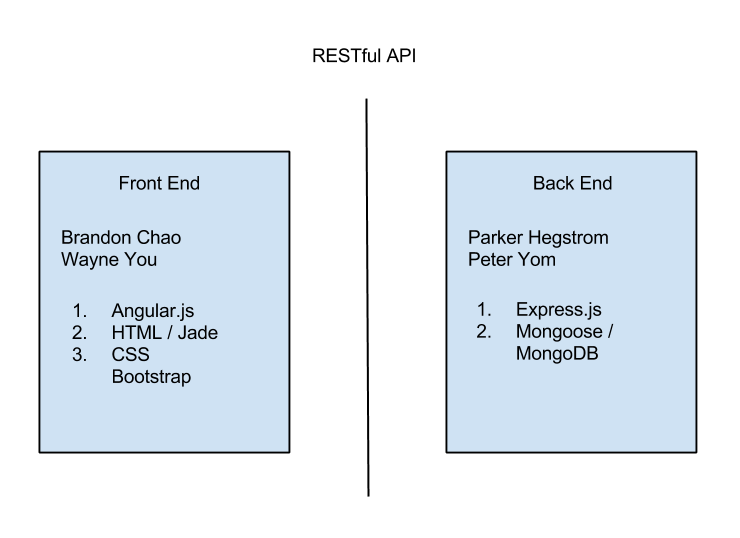
\includegraphics[width=.5\textwidth]{DesignDiagram.png}
\caption{Diagram of our Large Scale Design}
\label{design}
\end{figure}

\noindent Essentially, our back end team provides an exhaustive RESTful API service to our front end. As we received the new requirements for evolution two, the benefits of our modular design came to light as we met to discuss both the refactorings from evolution one that needed to be done and the edits to each modules system design in order to account for the added calendar functionality--event requests and persistent until done events.\\

\noindent At the beginning of evolution two, our group spent four days simply refactoring and making large design change decisions. The back-end did not undergo much broad change, but the front end implemented a new type of calendar (see Front End Section for further analysis on this). Our modular design has been engineered in such a way that any front end client service can use our backend service. Because of this, development on the backend did not have to stop and integration of the new front end was seamless.\\

\noindent The following sections further discuss design choices and implications of those design choices for both our front end and back end teams. \\

\section{Back End Design and Analysis}
\subsection{New Features}

\dcomment{Dont write backslashes, just put a blank line between paragraphs.  If you want to adjust the spacing, set parskip.}

The back-end introduced sharing on an event granularity through event invitation, request objects, and PUDs.  Also, we introduced a powerful new tool called deepPopulate.

\noindent DeepPopulate is a mongoose plugin that allows us to do deep population of nested models.  During the development of evolution 1, we were unable to deep populate and instead resorted to levels of callbacks on callbacks in a ham\dcomment{-}fisted attempt to populate down more than 1 level of a mongoose model.  For example, when returning a Calendar to the front end, we would first query for a user, populate its calendars, and for each Calendar we would query for the events, owner, and rules within callbacks and add them to the JSON object to return.  We could continue deep populating this way, but the levels of callbacks made the code incredibly challenging.  DeepPopulate allowed us to populate multiple fields from a model at whatever depth we desired in 1 line.  This sped up production and gave us incredible flexibility in how we package information to send to the front end.

\noindent While designing requests and redesigning events, we realized that they are very much tied together.  When a new event is created, a matching request object is also created alongside it.  This request object holds all of the information about which users have been invited to edit the event and their statuses: pending, accepted, denied, rejected.  When a user is invited to an event, the \_id for the request is added to the user's 'eventRequest' field.  The requests in a user's \dcomment{'}eventRequest' field are all of the pending requests that the user must respond to.  Upon accepting a request, a copy of the original event is created and placed in the calendar of the accepting user's choosing.  This copy is a stand alone event with similar information to the original event.  That way, when an edit is made to the original event, the copy is not altered until the user accepts the edits.

\noindent The ability to create an event that is persistent until done (PUD) was another major addition in functionality to the calendar. At first, we wanted to try \dcomment{to} reuse our Event schema to handle the PUDs, but one of the requirements (requirement g) forced us to decouple them. Hence, we created a new model for the PUD completely \dcomment{(elaborate?)}. \\

\noindent Although we were not able to completely reuse the code from the Event, we were able to reuse the Alert type we created in the first evolution with some minor additions to the schema definition. This allowed us to call our Alert constructor when a PUD event was created and email handling would happen automatically without any changes (email handling happens in {\tt alertRoutes.js}. Apart from some refactorings to make the code cleaner, this file did not change much.\\

\noindent PUDs can also be set to repeat at a certain interval (we elected to allow the user to select this repeat on the a day count granularity, 7 would be for weekly). The {\tt repeatInterval} property in the PUD schema held this information and is set upon creation. Upon completion, our server code checks to see if an interval has been set. If so, the {\tt date} property is updated accordingly and the PUD is \dcomment{preserved} in the database. This PUD will not appear on the users To-Do list until this new date, because the GET request for the To-Do section filters out any date that does not precede the current time.

\subsection{Benefits of Our Previous Design}

Our previous design worked well for what it was intended to do.  Everything was functional and robust, albeit a bit messy and cluttered in the code at times.  However, the modular way in which we organized our routes allowed us to very easily add new functionality to our old code.  Unless we were explicitly re-designing a section of the code, altering one part of the code did not affect the rest of the code.

\subsection{Drawbacks of Our Previous Design}

Our previous design had event sharing on a calendar granularity.  For example, one event was fixed to one calendar, but the entire calendar could be shared with another user.  Unfortunately, the new evolution required us to be able to share and invite single individual events.  In order to fulfill this requirement, we had to redesign our event schema and how calendars store events.  It was not a painful fix, but it was definitely took some redesigning and rethinking of our calendar's functionality.\\

\noindent Our previous design also worked around our lack of understanding of deepPopulate and promises.  There were several areas with multiple levels of nested callbacks and re-routing in order to work around our problems.  However, in this evolution, we learned how to properly deepPopulate and to utilize promises.  These new developments helped clean up our code, decrease development time, and gave us incredible flexibility and control over our mongoose queries, how we package and populate data, and the overall flow of our code.\\

\section{Front End Design and Analysis}

\noindent The web client required a number of additional functions in order to handle requests and PUD events. Thanks to the modularity of the previous design, most of these additional functions did not require many changes to existing code. This allowed more time to refactor existing code and provide many quality of life upgrades.\\

\noindent PUD events were added in as an additional list retrieved from the server. We displayed them using an Angular repeating list in the sidebar by replacing the previous location for local calendar events. The sidebar was almost out of space for an additional section, and the current design will require a significant UI overhaul if we must add any more sections for the sidebar. In order to display PUD events inside of calendar events, we simply added a section for display in the event detail display that becomes populated via a GET when the event is selected. We could potentially use this method to get more data in the future, but the more data we need to retrieve from the server, the slower the detail modal will load.\\

\noindent Requests were added as a paired object with events. Each event creates an empty request during creation which can be populated by a new form. These requests are shown in a sidebar region that shows sent requests and received requests as well as any updates to sent requests. Requests do not update immediately on other clients and require a refresh to update when sent out.\\

\noindent The rest of the code changes involved refactoring large functions, organizing the code more logically, implementing modals for UI experience, providing more auto-filled inputs, and caching data locally. The lingering problems in the design after these changes are the overuse of \$rootScope (a global scope for Angular) and the increasing size of our modal controller. The first problem is due in part to the scoping of Angular. If we wish to pass a value from one scope to another, it is impossible without passing it through the root scope. However, the root scope does not actually have knowledge of any of its child scopes, so the data passed must be stored in a global scope in order to transfer. The other problem of the scope of the modal controller can be fixed by decomposing the controller since the constituent parts are very loosely connected.\\

\noindent The choice of caching and updating the data locally in conjunction with database updates has come with some benefits and some detriments. For user experience and future use, keeping and updating the data locally drastically reduces the \dcomment{number} of GET requests sent and parsed to maintain data consistency. However, this \dcomment{reduction} comes at the cost of increasing the code considerably for the client. Instead of requesting and re-displaying all of the data, the data on local copies must be manually updated to ensure that the user sees values consistent with the database. This will add to development time in the future.\\

\noindent Finally, the Jade template for our single-page site has been growing considerably. Almost all of the relevant HTML for the calendar page is within a single file. If possible, the created modals may need to be moved into their own HTML files, and the sidebars should be converted into UI routes for Angular to better organize the HTML. As it is now, future development will become harder the more we are required to sift through the file for details.\\

\section{Individual Portion}
\subsection*{Parker}

\begin{enumerate} [a)]
\item  {\bf Designing and Conducting Experiments}
\begin{enumerate} [$\cdot$]
\item A special feature of javascript in general is that it is asynchronous. To deal with this asynchronous nature of the code, callback functions are used. However, multiple callback functions with callback functions (also known as callback hell) makes it harder to find bugs and/or simply read the code. I researched the use of promises alongside mongoDB and Mongoose. After researching, I then tested the promise implementation--accessing the database with a promise and utilizing the exposed promise API. Minor kinks were worked out, but Peter and I were able to clean up some of our code with promises from then on. \dcomment{(this describes research, but not so much an experiment).}
\end{enumerate}
\item  {\bf Analyzing and Interpreting Data}
\begin{enumerate} [$\cdot$]
\item At times, router methods we wrote did not behave properly, and by that I mean that certain errors were thrown to the console. Different HTTP error codes made up the majority of these errors, so I had to interpret what the server was telling me in order to both find the problem and determine what the best solution would be. One example of this that comes to mind was a server 500 response we were getting from issuing a PUT to the {\tt /pud/reorder} endpoint. After analyzing more console outputs, I was able to find that the Express router treats {\tt /pud/reorder} and {\tt /pud/:pudID} (which is a query parameter) as the same, so both routes were being run \dcomment{(strange?)}. 
\end{enumerate}
\item {\bf Designing System Components}
\begin{enumerate} [$\cdot$]
\item One new component I designed in the back-end was the PUD. We, as a group, wanted to integrate the PUD into the overall project and specific events without much change to existing code. With that in mind, I made the PUD a separate document type in our database, BUT it shared some of the pre-existing functionality we had developed for alerts and repeats. I was able to reuse a lot of code by using the �populate� \dcomment{(Im not sure what the weird chars are for here?)} as well as the Alert schema to handle such things. An interesting requirement for the PUD was that you could set a time interval (i.e. weekly for the repeat), yet, once the PUD was marked complete, you wouldn�t want it to immediately show up in the list of outstanding PUDs. This was solved by editing the �GET /pud� method to check the {\tt createdDate} for each PUD. 
\end{enumerate}
\item {\bf Dealing with Realistic Contraints}
\begin{enumerate} [$\cdot$]
\item As I stated in the previous design document we submitted, javascripts asynchronous nature continued to prove difficult at times. Specifically, problems arose when we began writing more functions both in our route files and in our schema files rather than rewriting code all over the place. Each time we made a call to the database, the value would have to be returned to a callback function, so as we segregated our code more and more, we continued to have to abide by the callback rules of javascript, slowing our development speed tremendously at times.
\end{enumerate}
\item  {\bf Teamwork and Team Member Interaction}
\begin{enumerate} [$\cdot$]
\item Peter and I worked very \dcomment{closely} together on the backend, and, as a whole, I thought our group worked much better together than we did through the first evolution. I was able to work on new features concurrently with the rest of the group, meeting occasionally to make sure there were no design misunderstandings or any small typo-like bugs that would cause integration problems down the development path.
\end{enumerate}
\end{enumerate}

\subsection*{Wayne}

\begin{enumerate} [a)]
\item  {\bf Designing and Conducting Experiments}
\begin{enumerate} [$\cdot$]
\item Since the new changes to the calendar were not very intensive, I was able to spend more of my time learning how the server handled the HTTP requests during my debugging. While I was previously able to use the console to check the data sent in each request, I was unable to determine exactly what the server requested in some methods and how it was parsed. This led to some problems with Javascript lack of typing, and with this evolution, I was able to better tailor the HTTP requests that I wrote to send data without needing to confer with Parker and Peter on all of the details.
\end{enumerate}
\item  {\bf Analyzing and Interpreting Data}
\begin{enumerate} [$\cdot$]
\item One problem that was solved relatively quickly thanks to some discussion and better understanding of Javascript as a whole came about from sending a request accept. The request body sent an object which contained a calendar ID field, and checking the sent data never seemed to show why the accept constantly failed. After doing some server logging, it became apparent that the problem was the the field sent was CalID, and the field requested was calID, and Javascript went ahead and crashed the server on accessing an undefined value.
\end{enumerate}
\item {\bf Designing System Components}
\begin{enumerate} [$\cdot$]
\item I worked on the Event Request/Invites handling for this iteration as well as the PUD sidebar list. Request handling was mostly isolated except for two changes for events. The first change was manually adding an event into the calendar when an event was accepted, and the second was displaying a related request's details inside of an event's details. These changes were very easy, but they shared very similar code to existing functions. It may be to our benefit in the future to create more generalized functions and pass in particular parameters to them in order to reduce redundant functionality.
\end{enumerate}
\item {\bf Dealing with Realistic Contraints}
\begin{enumerate} [$\cdot$]
\item We moved away from the previous calendar implementation to an Angular implementation because the previous calendar only supported URL redirects or a single type of modal for event display. By switching to the Angular calendar, we were able to call a Javascript function that could provide more functionality. Also, Javascript has continued to be a frustrating language to deal with due to its loose object definitions and lack of typing. Many times a bug has been a spelling error leading to an undefined error that masks the source of the problem, and all debugging requires printing out the objects in question to determine if certain fields exist or if the object itself even exists.
\end{enumerate}
\item  {\bf Teamwork and Team Member Interaction}
\begin{enumerate} [$\cdot$]
\item We were able to meet much more often for this evolution and were able to work out details relatively quickly. The back-end team of Peter and Parker worked out most of the design for the objects being stored as well as the API. Brandon and I worked out the changes to the client, and we were able to continue to work mostly independently for this evolution as well.
\end{enumerate}
\end{enumerate}

\subsection*{Brandon}

\begin{enumerate} [a)]
\item  {\bf Designing and Conducting Experiments}
\begin{enumerate} [$\cdot$]
\item As we were refactoring our calendar, one change we made was to allow the user to select User Groups by name and Users by email instead of using their ID. This required changes to the back-end routes as well as the front-end to connect and display it on the calendar. When the back-end first implemented it, we found that the elements were not updating in live time as we added them through UI interaction. This was strange because once we refreshed the page, the elements in question would then display. I used console logging to examine the data objects before and after refreshing and found that we weren't updating the front-end object stored in the \$scope in Angular. As such, it wouldn't update correctly at first until we refreshed and the data was correctly populated using a GET from the back-end. To fix this, we had the back-end return the necessary object on the POST which we used to update the \$scope variable immediately. This caused Angular to re-render and display the data as expected.
\end{enumerate}
\item  {\bf Analyzing and Interpreting Data}
\begin{enumerate} [$\cdot$]
\item One thing that was causing problems was the object that the Calendar data was returned to us on the front-end versus the object that we used to pass into the Angular Calendar we were using. These are slightly different since the Angular Calendar requires some extra fields so we made a wrapper around the back-end Calendar object. Because of this \dcomment{wrapper (?)}, when we were redesigning the display for a section, we mixed up the two objects which caused the calendar application to not render correctly since it was missing data. This was solved by looking through the database objects for the calendars and comparing that to the log of the objects before and after refreshing the page. We soon found that we were setting the wrong object on the front-end for the Angular Calendar and a small change fixed the problem.
\end{enumerate}
\item {\bf Designing System Components}
\begin{enumerate} [$\cdot$]
\item One new component I worked on for this iteration was PUD. Wayne implemented a solid design for it using Angular and I worked mainly on integrating the UI with the existing parts of the project. To do this, I redesigned select parts of the dashboard.jade file to make the code more modular and readable and to display more cleanly in our application. However, one other thing I would like to do soon in the future is to pull out the modal html files into separate files to make the dashboard even more concise.
\end{enumerate}
\item {\bf Dealing with Realistic Contraints}
\begin{enumerate} [$\cdot$]
\item One constraint I had to deal with is our use of the Angular Bootstrap Calendar. Although it is definitely more flexible than the previous calendar implementation we were using, since we did not design it from scratch, we are still somewhat dependent on how the creator of the Angular Calendar implemented its API. For example, since the whole calendar is added in our page as one element, it is difficult to make specific changes to it that are not supported by the Calendar's API. I wanted to add more user interaction functionality such as allow doubling clicking to create events, or adding in various elements to the imported calendar display, but in order to do these, it would require us to either modify the source code of the calendar or implement the changes in a hacky way using the available API calls to the calendar. In the future, I hope to find a way around this so we can add more features and alter the calendar to our liking more specifically.
\end{enumerate}
\item  {\bf Teamwork and Team Member Interaction}
\begin{enumerate} [$\cdot$]
\item We met up more frequently and earlier in the evolution and thus were able to set team goals and priorities much earlier. As a result, we were able to wrap up the functionality portion of evolution 2 on time and had extra time to update the UI and refactor our code. Wayne and I worked well together on the client-side.
\end{enumerate}
\end{enumerate}

\subsection*{Peter}

\begin{enumerate} [a)]
\item  {\bf Designing and Conducting Experiments}
\begin{enumerate} [$\cdot$]
\item The asynchronous nature of javascript has been both a very powerful feature and an absolute nuisance for our group.  During the development of evolution 1, Parker and I tried several work arounds of javascript's asynchronous callback functions.  With our workarounds with nested callbacks and whatnot, our code was functional but becoming increasingly messier and harder to read.  While refactoring the code base for evolution 2, we decided to go more in depth with \dcomment{'}promises'.  I did research on promises, tested the functionality of promises, and ultimately added promises to the code in order to clean up what we called 'call-back hell'. \dcomment{(this describes research, but not so much an experiment).}
\end{enumerate}
\item  {\bf Analyzing and Interpreting Data}
\begin{enumerate} [$\cdot$]
\item Javascript's asynchronous nature gave us a few headaches here and there.  At one point, the front end would call a route, but the route was running multiple times.  Every time this route would be called, the server would return the necessary data back to the front end and then crash.  The reason for the crash was because the route was running multiple times, the header would be set multiple times as well.  After carefully playing with the code, trying a few work arounds with counters, and searching, I eventually found a level in a schema where it was calling callbacks in a loop.  Upon fixing this issue, the route worked perfectly.
\end{enumerate}
\item {\bf Designing System Components}
\begin{enumerate} [$\cdot$]
\item I designed a large portion of how event request invites function.  I created a new schema for a {\tt Request} object.  Each {\tt Request} object is associated with an {\tt Event} object and vice versa.  When a new {\tt Event} is created, a matching {\tt Request} is also initiated, because I realized that each event can have multiple event requests stemming out from it.  Key elements of the {\tt Request} schema are a reference to the original {\tt Event} it stems from, an array of all of the user ids that the original creator has invited to the request, an array of those each invited user and their status (pending, accepted, rejected, etc), and an array of edits to the {\tt Event}.  When an invited user accepts a pending request, he creates a copy of the original event and adds it to one of his calendars.  That way, if the original creator of the event edits the event, the copied event is not altered until the user re-accepts the changes.
\end{enumerate}
\item {\bf Dealing with Realistic Contraints}
\begin{enumerate} [$\cdot$]
\item Javascript's asynchronous nature made it so that some routes would send a response back before parts of the route code would complete.  This was a nightmare to deal with, but we fixed this problem by looking into promises.  Promises allowed us to dictate that certain parts of the code could not be entered until specific parts of the code had been completed.  With promises, we became much more in control of how our code works.
\end{enumerate}
\item  {\bf Teamwork and Team Member Interaction}
\begin{enumerate} [$\cdot$]
\item Our group was much more cohesive and organized than we were for evolution 1.  We were able to plan out meetings ahead of time, hash out design details earlier, and finished all of our evolution 2 requirements with time to spare.  As usual, Parker and I met often as the back-end team very often. 
\end{enumerate}
\end{enumerate}

%\keywords{Cremona map \and Newton complementary dual \and monoid \and Cohen--Macaulay}

%\vspace{0.2in}




%\begin{align}
%e^{j\theta} = cos(\theta) + jsin(\theta)
%\end{align}

%\begin{figure}[h]
%\begin{center}
%\epsfig{file=StatPlot.eps, width=5in}
%\caption{\label{boxplot} Box plot of the survey data}
%\end{center}
%\end{figure}


%\begin{figure}[h]
%\begin{center}
%\epsfig{file=histogram.eps, width=4in}
%\caption{\label{histogram} Histogram plot of the survey data}
%\end{center}
%\end{figure}

%\begin{table}[h]
%\begin{center}
%\caption{\label{histotable}Table of frequency values from the Histogram} 
%\begin{tabular}{|c|c|}\hline
%{\bf Type of Engineering} & Frequency \\
%BME & 59 \\
%CEE & 6 \\
%ME & 3 \\
%ECE & 10 \\
%Undecided & 1 \\ \hline
%\end{tabular} \\~\\
%\end{center}
%\end{table}

%\begin{figure}[htb]
%\centering
%\includegraphics[width=1.3\textwidth]{Screenshot.png}
%\caption{Screen shot from StatKey}
%\label{samples}
%\end{figure}


%\appendix
%\section{Codes}
%\subsection{MakeGraph.m}
%\listinginput[1]{1}{MakeGraph.txt}


% GIVES TWO TABLES BY EACHOTHER
%\begin{table}[h!]
%\begin{minipage}[b]{0.45\linewidth}\centering
%\caption{\label{ecoli3}Using {\tt ecoli\_edit\_120481.txt}} 
%\begin{tabular}{|c|c|c|}
%\hline
%1 & 1 & 1 \\
%\hline
%\end{tabular}
%\end{minipage}
%\hspace{0.5cm}
%\begin{minipage}[b]{0.45\linewidth}
%\centering
%\caption{\label{ecoli4}Using {\tt ecoli\_edit\_3947161.txt}} 
%\begin{tabular}{|c|c|c|}
%\hline
%1 & 1 & 1 \\
%\hline
%\end{tabular}
%\end{minipage}
%\end{table}



\end{document}
% end of file template.tex

